\documentclass{article}

\usepackage{tabularx}
\usepackage[table]{xcolor}
\usepackage{multirow}

\usepackage{graphics}
\usepackage{graphicx}

\usepackage{listings}
\usepackage{xcolor}
\usepackage{color}

\usepackage{amsmath, amssymb}
\usepackage{mathtools}
\usepackage[margin=1.1in,footskip=.25in]{geometry}

\usepackage[most]{tcolorbox}

\tcbset{
    frame code={}
    center title,
    left=10pt,
    right=10pt,
    top=10pt,
    bottom=10pt,
    colback=gray!5,
    colframe=gray,
    width=\dimexpr\textwidth\relax,
    enlarge left by=0mm,
    boxsep=5pt,
    arc=0pt,outer arc=0pt,
    }

\renewcommand{\baselinestretch}{1.3} 

\definecolor{dkgreen}{rgb}{0,0.6,0}
\definecolor{gray}{rgb}{0.5,0.5,0.5}
\definecolor{mauve}{rgb}{0.58,0,0.82}
 
\definecolor{codegreen}{rgb}{0,0.6,0}
\definecolor{codegray}{rgb}{0.5,0.5,0.5}
\definecolor{codepurple}{rgb}{0.58,0,0.82}
\definecolor{backcolour}{rgb}{1,1,1}
 
\lstdefinestyle{mystyle}{
    backgroundcolor=\color{backcolour},   
    commentstyle=\color{codegreen},
    keywordstyle=\color{magenta},
    numberstyle=\tiny\color{codegray},
    stringstyle=\color{codepurple},
    basicstyle=\ttfamily\large,
    breakatwhitespace=false,         
    breaklines=true,                 
    captionpos=b,                    
    keepspaces=true,                 
    numbers=left,                    
    numbersep=5pt,                  
    showspaces=false,                
    showstringspaces=false,
    showtabs=false,                  
    tabsize=3
}

\lstset{style=mystyle}

\usepackage{xepersian}
\settextfont[Scale=1]{Vazir}

\begin{document}
\title{مهندسی اینترنت}
\maketitle

\begin{enumerate}
\item    دو مزیت اصلی معماری TCP/IP را شرح دهید ؟

\begin{tcolorbox}
\begin{itemize}
	\item یکی از قابلیت های عمده TCP/IP
	، امکان  اتصال شبکه ها به یکدیگر جهت ایجاد یک شبکه وسیعتر می باشد .
	
	\item در معماری TCP/IP
	هیچ استاندارد و پروتکل خاصی برای لایه های اول و دوم وضع نشده است، این امر باعث می شود که به راحتی بتوان از 
	TCP/IP
	بر روی فناوری های مختلف لایه فیزیکی استفاده کرد .
\end{itemize}
\end{tcolorbox}

\item کاربرد هر یک از کلاس های آدرس IP را توصیف نمایید ؟

\begin{tcolorbox}
\begin{itemize}
	\item کلاس A برای شبکه های خیلی بزرگ مناسب است
	، اما چون فیلد مشخص کننده شبکه ی آن فقط 7 بیت است، تنها 127 تا از چنین شبکه هایی قابل ایجاد می باشد
	
	\item شبکه های کلاس B شبکه هایی با اندازه متوسط هستند که برای سازمانهای متوسط و بزرگ مناسب  است 
	
	\item شبکه های کلاس C برای سازمان های کوچک مناسب اند ، در شبکه های کلاس
	 C نمی توان بیش از 
	254 میزبان داشت .
	
	\item کلاس D برای عملیات چندپخشی رزرو شده است 
	
	\item کلاس E برای استفاده های آینده رزرو شده است 
	
\end{itemize}
\end{tcolorbox}

\item مزایا و عیب های تقسیم آدرس IP به یک netid و hostid را چیست ؟

\begin{tcolorbox}
\begin{itemize}
	\item مزیت استفاده از مدل دو بخشی آدرس شبکه و آدرس میزبان برای آدرس های IP
	، کمینه کردن تعداد ورودی ها در جدول مسیریابی است .
	به جای اینکه برای هر میزبان در یک شبکه یک رکورد در جدول مسیریابی داشته باشیم، میتوان با استفاده از یک رکورد همه ی میزبان ها را در یک شبکه خلاصه کرد که فقط شامل قسمت آدرس شبکه است که پیشوند مشترک برای همه ی میزبان های شبکه می باشد .
\end{itemize}
\end{tcolorbox}


\newpage

\item کاربرد آدرس IP \lstinline{0.0.0.0} و  \lstinline{255.255.255.255} چیست ؟

\begin{tcolorbox}
\begin{itemize}
	\item [$0.0.0.0$] در این آدرس
	فیلد شماره شبکه صفر است که به معنی این شبکه می باشد ، فیلد شماره میزبان نیز صفر است که به معنی این نود در شبکه می باشد ، این آدرس معمولاً زمانی استفاده می شود که یک نود شبکه سعی می کند تا آدرس IP خود را مشخص کند .
	\item [$255.255.255.255$] این آدرس
	نشان دهنده ی یک آدرس همه پخشی محدود است که از 
	جانب مبدا به همه ی نود های آن شبکه ارسال می شود .
	همه پخشی محدود در شبکه های محلی قابل استفاده است و هرگز از مرز یک مسیریاب عبور نمی کند .
\end{itemize}
\end{tcolorbox}

\item نوع کلاس IP آدرس های زیر را به دست آورید ؟\begin{lstlisting}
23.1.3.5     198.34.54.23     233.12.3.4 
45.2.3.67     178.11.23.5     254.12.34.5 
\end{lstlisting}


\begin{tcolorbox}
\begin{align*}
23.1.3.5 &\to 00010111.00000001.00000011.00000101 \Rightarrow class \:\: A \\
198.34.54.23 &\to 11000110.00100010.00110110.00010111 \Rightarrow class \:\: C \\
233.12.3.4 &\to 11101001.00001100.00000011.00000100  \Rightarrow class \:\: D \\
45.2.3.67 &\to 00101101.00000010.00000011.01000011  \Rightarrow class \:\: A \\
178.11.23.5 &\to 10110010.00001011.00010111.00000101 \Rightarrow class \:\: B \\
254.12.34.5 &\to 11111110.00001100.00100010.00000101 \Rightarrow class \:\: E \\
\end{align*}
\end{tcolorbox}


\item عملکرد پروتکل NAT را توضیح دهید ؟

\begin{tcolorbox}
\begin{itemize}
	\item سیستم NAT آدرس های IP 
	شبکه ی محلی را به آدرس های یکتا برای استفاده بر روی اینترنت تبدیل می کند . هرچند این روش برای ایجاد آدرس های بیشتر برای استفاده در شبکه داخلی ابداع شده است ، ولی می توان از آن برای مخفی کردن اطلاعات مربوط به سیستم های داخلی نیز استفاده کرد .
	
	\item عملکرد NAT
	به این صورت است که یک دستگاه ( مثل کامپیوتر یا مسیریاب ) به عنوان دروازه ی ورود به اینترنت عمل می کند و شبکه ی داخلی را از دید اینترنت پنهان می کند ، از سوی دیگر اینترنت کل شبکه را به صورت یک دستگاه ساده میبیند که به اینترنت متصل می باشد .
\end{itemize}
\end{tcolorbox}



\newpage

\item پدیده ی ROADS را توضیح دهید ؟

\begin{tcolorbox}
\begin{itemize}
	\item آدرس های کلاس A و B
	به سرعت در حال تمام شدن می باشند که به این موضوع پدیده ی ROADS  می گویند .
\end{itemize}
\end{tcolorbox}

\item یک آدرس برگشت حلقه نرم افزاری چیست ؟ و چند نمایش آدرس برگشت حلقه وجود دارد ؟

\begin{tcolorbox}
عدد 127 در هشت بیت اول آدرس IP
که در بازه ی مقادیر کلاس A می باشد . در مجموعه آدرس های کلاس A استفاده نمی شود بلکه برای قابلیت برگشت حلقه رزرو شده است .

در خیلی از کاربردهای شبکه، تمایل به بررسی و تست نرم افزار و سیستم عامل شبکه می باشد .
نتایج موجود در هر بسته ای که توسط برنامه ی کاربردی به آدرس 
$127.0.0.0$
ارسال می شود، بدون دستیابی به واسطه ی شبکه به برنامه ی کاربردی بر می گردد .
به این دلیل این آدرس، آدرس برگشت حلقه نامیده می شود .
\end{tcolorbox}

\item مزایای زیر شبکه سازی را بنویسید ؟

\begin{tcolorbox}
\begin{itemize}
	\item کاهش ترافیک شبکه
	\item افزایش کارآیی شبکه
	\item ساده سازی مدیریت
	\item ساختار مدیریت
	\item ساختار دهی شبکه ی داخلی بدون تاثیر روی شیکه های خارجی
	\item بهبود بخشیدن به امنیت
\end{itemize}
\end{tcolorbox}

\item یک شبکه کلاس C با آدرس 
\begin{lstlisting}
194.34.56.0
\end{lstlisting}
داده شده است، چند میزبان برای  این شبکه وجود دارد ؟ 

\begin{tcolorbox}
\begin{align*}
194.34.56.0 \to \underbrace{11000010.00100010.00111000}_{Network}.\underbrace{00000000}_{Host}
\end{align*}

{
\LARGE
$$
2^{8} - 2
$$
}
\end{tcolorbox}

\newpage

\item یک شبکه کلاس B با آدرس 
\begin{lstlisting}
166.23.0.0
\end{lstlisting}
داده شده است، چند میزبان برای  این شبکه وجود دارد ؟ 

\begin{tcolorbox}
\begin{align*}
166.23.0.0 \to \underbrace{10100110.00010111}_{Network}.\underbrace{00000000.00000000}_{Host}
\end{align*}

{
\LARGE
$$
2^{16} - 2
$$
}
\end{tcolorbox}



\item مفهوم آدرس دهی تک پخشی، چند پخشی و همه پخشی را توضیح دهید ؟

\begin{tcolorbox}
\begin{itemize}
	\item هنگامی که یک بسته ی IP به یک IP
	انفرادی فرستاده می شود فرآیند ارسال تک پخشی نام دارد
	\item هنگامیکه یک بسته IP به همه نود های یک شبکه ی خاص فرستاده می شود ، فرآیند ارسال همه پخشی نام دارد 
	\item در فرآیند چند پخشی از یک کلاس آدرس D
	به عنوان آدرس مقصد استفاده می شود 
\end{itemize}
\end{tcolorbox}

\item آدرس کلاس A با چه عددی دودویی شروع می شود ؟ و محدوده ی آدرس این کلاس را مشخص کنید ؟

\begin{tcolorbox}
\begin{latin}
\begin{itemize}
	\item Class A :
\end{itemize}
\end{latin}
\begin{align*}
 0.  0.  0.  0 = &00000000.00000000.00000000.00000000 \\
127.255.255.255 = &01111111.11111111.11111111.11111111 \\
                  &0nnnnnnn.HHHHHHHH.HHHHHHHH.HHHHHHHH
\end{align*}
\end{tcolorbox}



\newpage

\item آدرس کلاس B با چه عددی دودویی شروع می شود ؟ و محدوده ی آدرس این کلاس را مشخص کنید ؟


\begin{tcolorbox}
\begin{latin}
\begin{itemize}
	\item Class B :
\end{itemize}
\end{latin}
\begin{align*}
128.  0.  0.  0 = &10000000.00000000.00000000.00000000 \\
191.255.255.255 = &10111111.11111111.11111111.11111111 \\
                  &10nnnnnn.nnnnnnnn.HHHHHHHH.HHHHHHHH
\end{align*}
\end{tcolorbox}


\item محدوده ی شبکه و میزبان را در کلاس های آدرس A و B و C مشخص کنید ؟


\begin{tcolorbox}
\begin{latin}
\begin{itemize}
	\item Class A :
\end{itemize}
\end{latin}
\begin{align*}
 0.  0.  0.  0 = &\underbrace{00000000}_{Network}.\underbrace{00000000.00000000.00000000}_{Host} \\
127.255.255.255 = &\underbrace{01111111}_{Network}.\underbrace{11111111.11111111.11111111}_{Host} \\
                  &0nnnnnnn.HHHHHHHH.HHHHHHHH.HHHHHHHH
\end{align*}



\begin{latin}
\begin{itemize}
	\item Class B :
\end{itemize}
\end{latin}
\begin{align*}
128.  0.  0.  0 = &\underbrace{10000000.00000000}_{Network}.\underbrace{00000000.00000000}_{Host} \\
191.255.255.255 = &\underbrace{10111111.11111111}_{Network}.\underbrace{11111111.11111111}_{Host} \\
                  &10nnnnnn.nnnnnnnn.HHHHHHHH.HHHHHHHH
\end{align*}


\begin{latin}
\begin{itemize}
	\item Class C :
\end{itemize}
\end{latin}
\begin{align*}
192.  0.  0.  0 = &\underbrace{11000000.00000000.00000000}_{Network}.\underbrace{00000000}_{Host} \\
223.255.255.255 = &\underbrace{11011111.11111111.11111111}_{Network}.\underbrace{11111111}_{Host} \\
                  &110nnnnn.nnnnnnnn.nnnnnnnn.HHHHHHHH
\end{align*}
\end{tcolorbox}

\newpage

\item مشخص کنید که آدرس 
\begin{lstlisting}
192.168.1.18/24
\end{lstlisting}
جزء کدام دسته کلاس آدرس می باشد و آدرس خود شبکه ، اولین میزبان ، آخرین میزبان و آدرس Broadcast را در این شبکه مشخص کنید ؟

\begin{tcolorbox}
$$
192.168.1.18 \to 11000000.10101000.00000001.00010010 \Rightarrow class \:\: C
$$

$$
\underbrace{192.168.1}_{Network}.\underbrace{18}_{Host}
$$


\begin{align*}
Subnet &= 192.168.1.00000000 \\
1st \:\: Host &= 192.168.1.00000001 \\
Last \:\: Host &= 192.168.1.11111110 \\
Broadcast &= 192.168.1.11111111 \\
\end{align*}

\end{tcolorbox}


\item مشخص کنید که آدرس 
\begin{lstlisting}
172.16.35.123/20
\end{lstlisting}
جزء کدام دسته کلاس آدرس می باشد و آدرس خود شبکه ، اولین میزبان ، آخرین میزبان و آدرس Broadcast را در این شبکه مشخص کنید ؟

\begin{tcolorbox}
$$
172.16.35.123 \to 10101100.00010000.00100011.01111011 \Rightarrow class \:\: B
$$


$$
\underbrace{172.16}_{Network}.\underbrace{35.123}_{Host}
$$


\begin{latin}
\begin{center}
  \begin{tabular}{ r  r | l  }
    Subnet $\to$ & 172.16.0010 & 0000.00000000 \\
    1st Host $\to$ & 172.16.0010 & 0000.00000001 \\
    Last Host $\to$ & 172.16.0010 & 1111.11111110 \\
    Broadcast $\to$ & 172.16.0010 & 1111.11111111 \\
  \end{tabular}
\end{center}
\end{latin}


\begin{latin}
\begin{center}
  \begin{tabular}{ r  l   }
    Subnet $\to$ & 172.16.32.0  \\
    1st Host $\to$ & 172.16.32.1  \\
    Last Host $\to$ & 172.16.47.254 \\
    Broadcast $\to$ & 172.16.47.255 \\
  \end{tabular}
\end{center}
\end{latin}

\end{tcolorbox}

\newpage

\item مشخص کنید که آدرس 
\begin{lstlisting}
172.16.129.1/17
\end{lstlisting}
جزء کدام دسته کلاس آدرس می باشد و آدرس خود شبکه ، اولین میزبان ، آخرین میزبان و آدرس Broadcast را در این شبکه مشخص کنید ؟

\begin{tcolorbox}
$$
172.16.129.1 \to 10101100.00010000.10000001.00000001 \Rightarrow class \:\: B
$$


$$
\underbrace{172.16}_{Network}.\underbrace{129.1}_{Host}
$$



\begin{latin}
\begin{center}
  \begin{tabular}{ r  r | l  }
    Subnet $\to$ & 172.16.1 & 0000000.00000000 \\
    1st Host $\to$ & 172.16.1 & 0000000.00000001 \\
    Last Host $\to$ & 172.16.1 & 1111111.11111110 \\
    Broadcast $\to$ & 172.16.1 & 1111111.11111111 \\
  \end{tabular}
\end{center}
\end{latin}



\begin{latin}
\begin{center}
  \begin{tabular}{ r  l   }
    Subnet $\to$ & 172.16.128.0  \\
    1st Host $\to$ & 172.16.128.1  \\
    Last Host $\to$ & 172.16.255.254 \\
    Broadcast $\to$ & 172.16.255.255 \\
  \end{tabular}
\end{center}
\end{latin}

\end{tcolorbox}

\item کاربرد و دلیل استفاده از پروتکل ARP را توضیح دهید ؟

\begin{tcolorbox}
\begin{itemize}
	\item از آنجاییکه در کامپیوتر مقصد، ابتدا لایه ی دوم قاب را از شبکه برداشته و بعد به لایه ی سوم که پروتکل IP 
	است تحویل می دهد ، لذا دانستن تنها آدرس IP مقصد کفایت نکرده و باید آدرس سخت افزاری کامپیوتر مقصد نیز داشته باشیم ، به این علت از پروتکلی به نام ARP استفاده می کنیم . 
	از پروتکل ARP 
	برای استخراج آدرس لایه سخت افزاری که به آن
	MAC-Address
	گفته می شود از آدرس IP استفاده می شود .
\end{itemize}
\end{tcolorbox}

\item محدودیت پروتکل ARP را توضیح دهید ؟

\begin{tcolorbox}
\begin{itemize}
	\item پروتکل ARP
	توسط پروتکل IP بسته بندی نمی شود ، بلکه مستقیماً توسط پروتکل لایه پیوند داده بسته بندی می گردد . این بدان معنی است که پیام های پروتکل ARP را نمی توان مسیریابی کرد، یعنی نمی تواند از مرز یک مسیریاب عبور کند .
\end{itemize}
\end{tcolorbox}



\newpage

\item به چه علت پیام درخواست ARP به صورت همه پخشی ارسال می شود ؟

\begin{tcolorbox}
\begin{itemize}
	\item در هنگام ارسال پیام درخواست ARP
	از آنجاییکه آدرس سخت افزاری مقصد هنوز معلوم نیست، بنابراین درخواست فوق در لایه ی دوم به صورت همه پخشی ارسال شده طوری که همه ی میزبان های شبکه بتوانند آن را دریافت کنند .
\end{itemize}
\end{tcolorbox}

\item آیا پیام پاسخ ARP به صورت همه پخشی ارسال می شود ؟ توضیح دهید ؟

\begin{tcolorbox}
\begin{itemize}
	\item پاسخ ARP 
	که توسط نود مقصد فرستاده می شود یک قاب همه پخشی نیست ، زیرا این نود آدرس سخت افزاری را در پیام درخواست ARP دریافت کرده است . بنابراین در هنگام پاسخ دهی ، قاب پاسخ را به صورت تک پخشی ارسال می دارد .
\end{itemize}
\end{tcolorbox}


\item چگونه آزمون آدرس IP تکراری ARP انجام می شود ؟

\begin{tcolorbox}
\begin{itemize}
	\item هر کامپیوتر در هنگام راه اندازی یک درخواست ARP
	را در شبکه منتشر می کند . در این پیام آدرس IP مقصد مساوی با آدرس IP فرستنده می باشد .
	در صورتی که فرستنده پاسخ پیام ARP 
	را دریافت کند ، بدین معنی است که نود دیگری با این آدرس موجود می باشد که به معنای وجود آدرس های IP تکراری در شبکه می باشد .
\end{itemize}
\end{tcolorbox}

\newpage

\item ساختار بسته های IPv4 را رسم کرده و کاربرد هر فیلد را توضیح دهید ؟

\begin{center}
	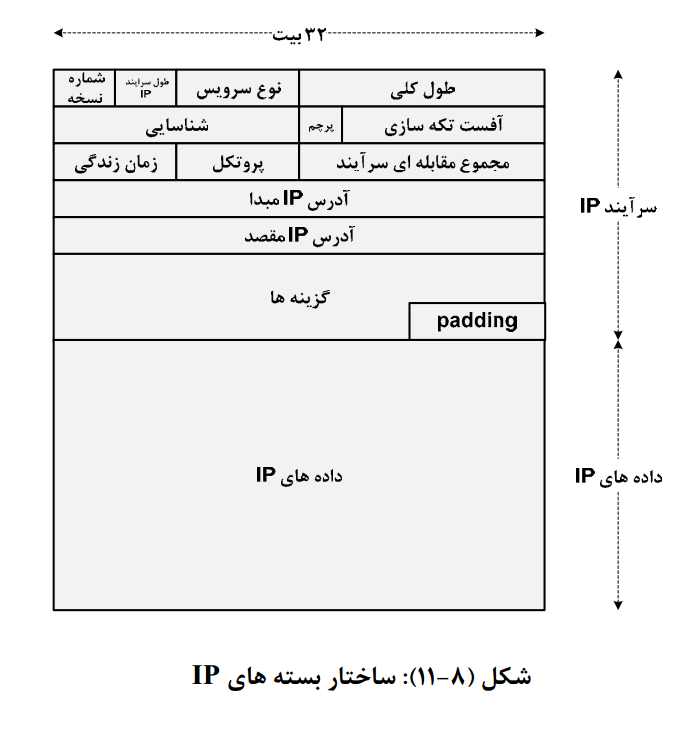
\includegraphics[scale=0.6]{./ip_1.png}
	%\caption{}
\end{center}

\item مفهوم MTU را توضیح دهید ؟

\begin{tcolorbox}
\begin{itemize}
	\item به حداکثر میزان  واحد قابل ارسال در یک شبکه ی فیزیکی ، حداکثر واحد ارسال 
	(MTU) 
	می گویند .
\end{itemize}
\end{tcolorbox}

\item کاربرد TTL را در بسته های IP بنویسید ؟

\begin{tcolorbox}
\begin{itemize}
	\item فیلد زمان زندگی که بر حسب ثانیه اندازه گیری می شود ، نشان دهنده ی حداکثر زمانی است که یک بسته IP 
	می تواند در شبکه زنده بماند .
	\item در هر مسیریاب میانی ، مقدار زمان لازم برای پردازش یک بسته از مقدار فیلد فوق کم می شود .
	\item 	هنگامی که مقدار فیلد TTL در یک بسته IP صفر می شود . یک پیام ICMP برای آگاهی از این حقیقت به مبدا فرستاده می شود .
	\item در صورت عدم وجود TTL 
	، پیام ها ممکن است در یک حلقه گیر کنند و باعث ترافیک زیاد در شبکه بشوند .
\end{itemize}
\end{tcolorbox}

\newpage

\item حداقل 5 مشکل را نام ببرید که از ICMP می توان برای گزارش دادن آنها استفاده کرد ؟

\begin{tcolorbox}
\begin{itemize}
	\item صفر شدن TTL
	\item عدم تحویل بسته به علت گم شدن یک تکه از بسته
	\item در دسترس نبودن یک پروتکل ، سرویس یا میزبان خاص در مقصد
	\item عدم توانایی پیش بردن یک بسته به خاطر عدم اجازه تکه سازی
	\item وقوع ازدحام در یک مسیریاب شبکه
\end{itemize}
\end{tcolorbox}

\item آیا ICMP در مورد بسته هایی که شامل پیام  ICMP هستند استفاده می شود یا خیر ؟ توضیح دهید ؟

\begin{tcolorbox}
\begin{itemize}
	\item پیام های ICMP
	برای اعلام وقوع خطا برای خود پیام های ICMP
	استفاده نمی شوند . زیرا پیام ها به شدت زیاد شده و به ترافیک شبکه اضافه می شود .
\end{itemize}
\end{tcolorbox}

\item منظور از فیلد های نوع و کد در یک پیام ICMP چیست ؟

\begin{tcolorbox}
\begin{itemize}
	\item فیلد نوع نشان دهنده ی نوع سرویس ICMP است
	\item فیلد کد اطلاعات بیشتری را درباره ی فیلد نوع به ما می دهد
\end{itemize}
\end{tcolorbox}

\item چه هنگامی پیام ICMP نوع 3 باید فرستاده شود ؟

\begin{tcolorbox}
\begin{itemize}
	\item هنگامی که یک مسیریاب قادر به تحویل بسته به مقصد نباشد
	یک پیام ICMP در دسترس نبودن مقصد با فیلد نوع 3 ارسال می کند . ( فیلد کد اطلاعات بیشتری را در مورد اینکه چرا مقصد در دسترس نیست نشان می دهد )
\end{itemize}
\end{tcolorbox}

\item دلایل ایجاد ازدحام در یک مسیریاب شبکه را توضیح دهید ؟

\begin{tcolorbox}
\begin{itemize}
	\item در شرایطی که حافظه یا ظرفیت بافر در مسیریاب های میانی شبکه برای ذخیره ی بسته های ورودی وجود نداشته باشد ، ازدحام به وجود می آید .
\end{itemize}
\end{tcolorbox}


\newpage

\item کاربرد پیام تغییر مسیر ICMP را توضیح دهید ؟

\begin{tcolorbox}
\begin{itemize}
	\item هنگامی که یک مسیریاب شبکه بسته ای را برای ارسال دریافت نماید ولی تشخیص دهد که مسیریاب دیگری مسیر بهینه تری برای ارسال بسته به سمت مقصد دارد ، 
	اقدام به ارسال پیام ICMP تغییر مسیر می نماید .
\end{itemize}
\end{tcolorbox}

\item در چه حالت هایی پیام ICMP تخطی از زمان فرستاده می شود ؟

\begin{tcolorbox}
\begin{itemize}
	\item هر گاه مقدار فیلد TTL در بسته های IP به صفر برسد 
	\item هرگاه یک تکه از بسته های IP
	 تکه شده طی زمان مشخصی به مقصد   نرسد ،
 مقصد یک پیام
	 ICMP تخطی زمانی 
	با مقدار کد 1 ارسال می کند
\end{itemize}
\end{tcolorbox}

\item چه زمانی پیام ICMP مشکل پارامتر ارسال می شود ؟

\begin{tcolorbox}
\begin{itemize}
	\item چنانچه مسیریاب متوجه مشکلی در پارامترهای سرآیند IP بسته های دریافتی شوند ،
	از پردازش بسته جلوگیری کرده و یک پیام ICMP 
	مشکل پارامتر ارسال می شود .
\end{itemize}
\end{tcolorbox}

\item در ساختار بسته های IP ، کاربرد فیلد نوع سرویس و اجزای آن را بنویسید ؟

\begin{tcolorbox}
\begin{itemize}
	\item فیلد نوع سرویس ، نوع سرویس درخواستی را از نظر پارامترهایی نظیر : 
	\begin{itemize}
		\item میزان تقدم
		\item تاخیر
		\item گذردهی
		\item اطمینان
	\end{itemize}
	  مشخص می کند
\end{itemize}
\end{tcolorbox}


\newpage

\item مزایا و معایب بازسازی بسته ها در مسیریاب های میانی شبکه را توضیح دهید ؟

\begin{tcolorbox}
\begin{itemize}
	\item عدم بازسازی تکه ها
	\begin{itemize}
		\item حمل بسته هایی تکه شده با اندازه کوچک باعث کاهش بازدهی پروتکل می شود .
		\item منجر به ترافیک زیاد در شبکه می شود 
		\item اگر یک تکه گم شود ، امکان بازسازی بسته اصلی نبوده و علیرغم انتقال موفق تکه های باقیمانده ، بسته اصلی باید حذف شود . با افزایش تعداد تکه ها ، احتمال از دست رفتن یک بسته IP نیز افزایش می یابد .
	\end{itemize}

	\item بازسازی تکه ها در مسیر یاب های میانی
	\begin{itemize}
		\item باعث ساده سازی مسیریابهای میانی شبکه می شوند .
	\end{itemize}

\end{itemize}
\end{tcolorbox}

\item چه هنگامی پیام  ICMP فرونشاندن مبدا فرستاده می شود ؟ چرا این پیام نباید توسط مسیریاب ها فرستاده شود ؟

\begin{tcolorbox}
\begin{itemize}
	\item هنگامی که یک مسیریاب متوجه پر شدن ظرفیت حافظه ی خود می شود ، برای کاهش درخواست ها و کاهش ازدحام شبکه با حذف بسته های ورودی اضافی و فرستاده پیام ICMP فرو نشاندن مبدا به فرستندهایی که بیشترین درخواست ها را می فرستد از آن می خواهد که سرعت ارسال اطلاعات خود را کاهش دهند .
\end{itemize}
\end{tcolorbox}


\item تحت کدام شرایط مسیریاب ها باید پیام های ICMP را تولید کنند ؟

\begin{tcolorbox}
\begin{itemize}
	\item هنگامی که یک مسیریاب شبکه بسته ای را برای ارسال دریافت نماید ولی تشخیص دهد که مسیریاب دیگری مسیر بهینه تری برای ارسال بسته به سمت مقصد دارد ، 
	اقدام به ارسال پیام ICMP تغییر مسیر می نماید .
	\item در شرایطی که حافظه یا ظرفیت بافر مسیریاب ها برای ذخیره ی بسته های ورودی کافی نباشد 
	اقدام به ارسال پیام فرو نشاندن مبدا می نماید .
	\item هنگامی که مسیریابی متوجه مشکلی در پارامتر های سرآیند IP بسته های دریافتی شوند ، پیام ICMP
	مشکل پارامتر ارسال می کنند .
	\item هنگامی که TTL یک بسته
	به صفر برسد ، مسیریاب پیام ICMP تخطی زمان می فرستد .
\end{itemize}
\end{tcolorbox}


\newpage

\item توضیح دهید آیا ضمانتی وجود دارد که پیام های ICMP تحویل داده شوند ؟

\begin{tcolorbox}
\begin{itemize}
	\item پیام های ICMP برای ارسال 
	از بسته های IP استفاده می کنند 
	، و چون پروتکل IP تحویل پیام ها را ضمانت نمی کند بنابراین ممکن است پیام های ICMP گم شده و یا به خاطر ازدحام در مسیریاب های میانی حذف شوند .
\end{itemize}
\end{tcolorbox}



\item ویژگی های اصلی TCP را نوشته و به اختصار توضیح دهید ؟

\begin{tcolorbox}
\begin{itemize}
	\item حمل داده پایه ای
	\item اطمینان
	\item کنترل جریان
	\item تسهیم سازی
	\item اتصال انتها به انتها
	\item تقدم و امنیت
\end{itemize}
\end{tcolorbox}


\begin{tcolorbox}
\begin{itemize}
	\item حمل داده پایه ای
	\begin{itemize}
		\item TCP توانایی حمل جریان پیوسته ای از بایت ها در هر دو جهت اتصال را دارد .
	\end{itemize}
	\item اطمینان
	\begin{itemize}
		\item یکی از ویژگی های TCP تحویل مطمئن داده ها
		به صورت انتها به انتها است . برای مهیا سازی اطمینان TCP برای جبران داده های خراب ، گم شده از مدل ارسال مجدد تصدیق مثبت استفاده می نماید . در TCP سگمنت های جدید تنها زمانی فرستاده می شوند که سگمنت های قبلی ارسال شده تصدیق شده باشند . 
		\item در TCP 
		فرستنده با ارسال هر سگمنت ، منتظر دریافت پیام تصدیق مثبت ( ACK ) از طرف گیرنده می باشد . اگر ACK
		در یک بازه زمانی معین دریافت نشود ، سگمنت قبلی دوباره ارسال می شود .
		\item در TCP
		از مکانیزم شماره گذاری رشته برای مرتب کردن سگمنت هایی که خارج از نوبت دریافت شده اند و یا حذف سگمنت های تکراری استفاده می شود .
		\item در TCP
		در صورت وقوع خرابی در سگمنت های دریافتی ، با استفاده از فیلد مجموع مقابله ای در سرآیند بسته های TCP 
		، مشکل رفع می شود .
	\end{itemize}
	\item کنترل جریان
	\begin{itemize}
		\item توسط مکانیزم کنترل جریان در TCP
		، مقدار داده ارسال شده توسط فرستنده همواره کنترل می شود .
		\item پروتکل TCP از مکانیزم پنجره ی لغزان
		برای پیاده سازی کنترل جریان استفاده می کند .
	\end{itemize}
	\item تسهیم سازی
	\begin{itemize}
		\item استفاده مشترک چندین فرآیند لایه کاربرد از امکانات TCP/IP ، 
		تسهیم سازی نام دارد .
	\end{itemize}
	\item اتصال انتها به انتها
	\item تقدم و امنیت
\end{itemize}
\end{tcolorbox}


\item دلیل استفاده از UDP را نوشته و با TCP مقایسه نمایید ؟

\begin{tcolorbox}
\begin{itemize}
	\item پروتکل TCP
	با فراهم ساختن یک سرویس اتصال گرا می تواند از تحویل مطمئن داده به مقصد اطمینان حاصل کند . در حالیکه پروتکل
	UDP
	بدون اتصال است و نمی تواند تحویل داده ها را تضمین نماید .
	\item UDP
	بسته گراست و بر خلاف TCP
	، سرباری برای باز کردن ، نگهداری و بستن یک اتصال ندارد .
	\item به خاطر سادگی و بالاسری کم UDP
	، تعداد زیادی از برنامه های کاربردی شبکه بر مبنای UDP
	طراحی شده اند .
\end{itemize}
\end{tcolorbox}


\newpage

\item در چه مواقعی بهتر است که از UDP استفاده کرد و در چه مواقعی از TCP ?

\begin{tcolorbox}
\begin{itemize}
	\item در مواقعی که نیاز است تا داده ها به یک برنامه کاربردی خاص در حال اجرا در یک ماشین فرستاده شود و یا در وضعیتی که نیاز است داده ها به صورت همه پخشی یا چند پخشی ارسال شوند ، از پروتکل UDP 
	استفاده می گردد .
	\item برخی از برنامه های کاربردی اینترنت نیاز به همه ی توانایی های TCP
	نداشته و فقط به یک پروتکل حمل ساده که بتواند برنامه های کاربردی را در کامپیوتر شناسایی کند و یک بررسی خطای ساده مهیا سازد ، نیاز دارند .
	\item مزیت UDP
	برای کاربردهای همه پخشی/چند پخشی است . به این صورت که در TCP
	اگر یک بسته همه پخشی باید به 1000 ایستگاه فرستاده شود ، فرستنده TCP باید 1000 اتصال را باز کرده و داده ها را به هر اتصال بفرستد و سپس 1000 اتصال را ببندد .
	سربار بازکردن این اتصالات بسیار بالاست .
	اما چنانچه از پروتکل UDP استفاده شود ، فرستنده می تواند داده را به ماژول IP با درخواست همه پخشی / چند پخشی بفرستد .
\end{itemize}
\end{tcolorbox}



\newpage

\item ساختار بسته های TCP را رسم نمایید ؟

\begin{center}
	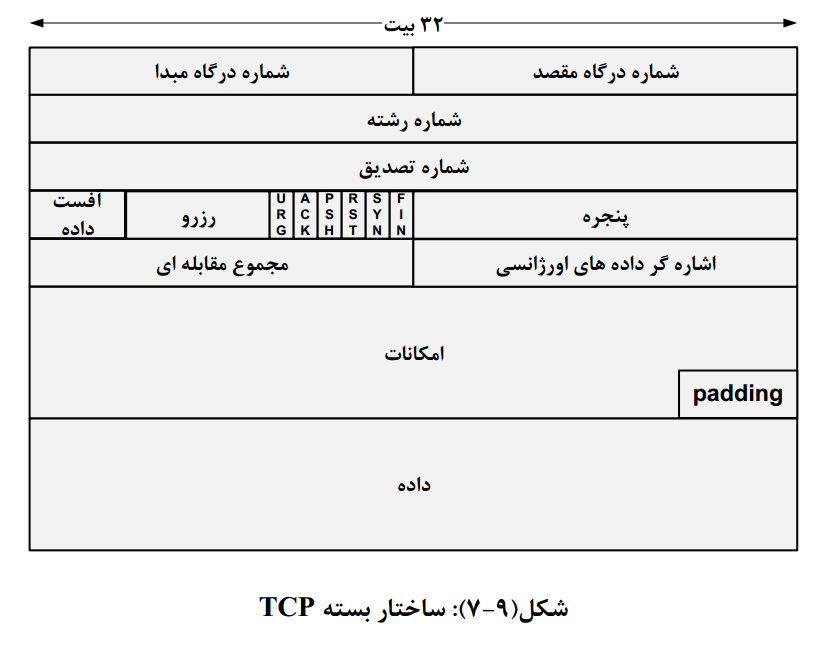
\includegraphics[scale=0.5]{./tcp_1.png}
	%\caption{}
\end{center}

\item کاربرد فیلد های شماره رشته ارسال و شماره تصدیق را در بسته های TCP توضیح دهید ؟


\begin{tcolorbox}
\begin{itemize}
	\item شماره رشته نشان دهنده ی اولین بایت داده در یک سگمنت TCP ارسالی می باشد .
	\item شماره تصدیق نشان دهنده ی  شماره بایتی است که فرستنده ، انتظار دریافت آن از طرف مقابل را دارد .
	\item به عنوان مثال ، اگر فیلد شماره رشته 100 باشد و فیلد شماره تصدیق 200 باشد ، بدان معنی است که بسته ارسالی از بایت 100 به بعد را شامل می شود و فرستنده تا بایت 199 را به طرف مقابل می فرستد و منتظر بایت 200 به بعد از طرف مقابل می باشد .
\end{itemize}
\end{tcolorbox}

\newpage

\item عملیات \lstinline{handshake} سه طرفه را توضیح دهید ؟

\begin{tcolorbox}
\begin{itemize}
	\item مبدا شماره رشته آغازین ( ISN ) ارسال خود را می فرستد
	\item  گیرنده، دریافت پیام فوق را با ارسال شماره تصدیق پاسخ می دهد . در اتصال های دو طرفه ، گیرنده نیز شماره رشته آغازین خود را به طرف مقابل می فرستد
	\item مبدا یک شماره تصدیق را برای تصدیق دریافت ISN ، می فرستد .
\end{itemize}
\end{tcolorbox}

\item کاربرد هر یک از پرچم های TCP را توضیح دهید ؟

\begin{tcolorbox}
\begin{itemize}
	\item [ACK] هنگامی که
	ACK
، 	1 باشد نشان می دهد که فیلد شماره تصدیق معتبر است .
	\item [SYN] برای نشان دادن باز شدن یک اتصال استفاده می شود
	\item [FIN] برای قطع یک اتصال استفاده می شود
	\item [RST] چنانچه در یک اتصال
	TCP
	خطای غیر قابل ترمیمی رخ دهد ، از بیت RST
	برای درخواست ری ست اتصال استفاده می شود .
	\item [PSH] وقتی این پرچم برابر با 1 شود
	گیرنده پیام باید فوراً آن را به لایه کاربرد تحویل دهد .
	\item [URG] از این پرچم برای ارسال فوری داده ها بدون انتظار کشیدن تا گیرنده بایت های قبلی در جریان را پردازش کند ، استفاده می شود 
\end{itemize}
\end{tcolorbox}

\item دلیل نامگذاری روش پنجره لغزان در TCP را توضیح دهید ؟

\begin{tcolorbox}
\begin{itemize}
	\item روش پنجره لغزان مکامیزمی است
	که مقدار داده ارسال شده توسط فرستنده را کنترل می کند
	\item لبه سمت چپ پنجره بیانگر کوچکترین شماره بایتی است که هنوز تصدیق نشده است . هنگامی که پیام تصدیقی برای داده های ارسال شده دریافت شد لبه پنجره می تواند به سمت راست حرکت کند . اندازه ی پنجره مقدار فضای در دسترس بافر در گیرنده را منعکس می کند .در صورتیکه گیرنده با ازدحام مواجه باشد ، بافر آن اغلب  پر می شود و بنابراین اندازه ی پنجره کاهش می یابد .
\end{itemize}
\end{tcolorbox}



\newpage

\item پدیده ی سندروم پنجره ی ابله را توضیح دهید ؟

\begin{tcolorbox}
\begin{itemize}
	\item در روش پنجره ی لغزان
	ممکن است بافر گیرنده فقط به اندازه ی یک بایت فضای خالی داشته باشد ، و به طرف مقابل خود اندازه پنجره یک بایتی را اعلام می نماید ، بدین ترتیب ، فرستنده قادر است فقط یک بایت داده را ارسال کند بنابراین اقدام به ارسال سگمنت های یک بایتی به طرف مقابل می نماید .
	با توجه به اینکه حداقل طول سرآیند TCP و IP هر کدام 20 بایت می باشد ، بنابراین برای ارسال 1 بایت داده بیش از 40 بایت سرآیند استفاده می شود که باعث کاهش شدید بهره وری در شبکه می شود . این پدیده سندروم پنجره ی ابله خوانده می شود .
\end{itemize}
\end{tcolorbox}

\item نحوه ی تعیین شماره رشته ی آغازین در یک اتصال TCP به چه صورت است ؟

\begin{tcolorbox}
\begin{itemize}
	\item در هنگام برقراری اتصال های TCP
	، پارامتری به نام شماره رشته آغازین ( ISN ) ، بین دو طرف مقابله می شود . ISN نشان دهنده ی شماره بایت اولین سگمنت ارسالی از هر طرف می باشد . مقدار فیلد ISN در صورتی معتبر است که مقدار پرچم SYN برابر با 1 باشد .
\end{itemize}
\end{tcolorbox}

\item مفهوم تسهیم سازی در TCP را توضیح دهید ؟

\begin{tcolorbox}
\begin{itemize}
	\item در پروتکل TCP 
	این امکان وجود دارد که به طور همزمان چندین سرویس ارتباطی بر روی یک کامپیوتر اجرا شود و همزمان داده های خود را برای ارسال به TCP تحویل می دهد .
	برای تفکیک این سرویس ها که از یک آدرس IP مشترک استفاده می کنند از شماره درگاه استفاده می شود .
	استفاده مشترک چندین فرآیند لایه کاربرد از امکانات TCP/IP ، تسهیم سازی نام دارد .
\end{itemize}
\end{tcolorbox}

\item مفهوم نقاط پایانی را در TCP توضیح دهید ؟

\begin{tcolorbox}
\begin{itemize}
	\item نقاط پایانی فرستنده ها یا گیرنده هایی هستند که از پروتکل TCP برای ارسال یا دریافت اطلاعات استفاده می کنند .
\end{itemize}
\end{tcolorbox}

\end{enumerate}

\end{document}